\section{Lessons Learned from the past}

\subsection{Data Independence}

Data independence means that the logical vew on the data is clearly separated, decoupled, from its physical storage. A relational database management system (RDBMS) exposes this logical model, together with logical building blocks for manipulating it, on top of a physical layer. A database management system stack can be viewed as a four-layer stack:
\begin{itemize}
    \item A logical query language with which the user can query data
    \item A logical model for the data
    \item A physical compute layer that processes the query on an instance of the model
    \item A physical storage layer where the data is physically stored.
\end{itemize}

\subsection{Relational Database Management Systems (RDBMS)}

\subsubsection{Formalism}

Definitions of the properties of a table can be seen in \cref{fig:table}.

\begin{figure}[h]
    \centering
    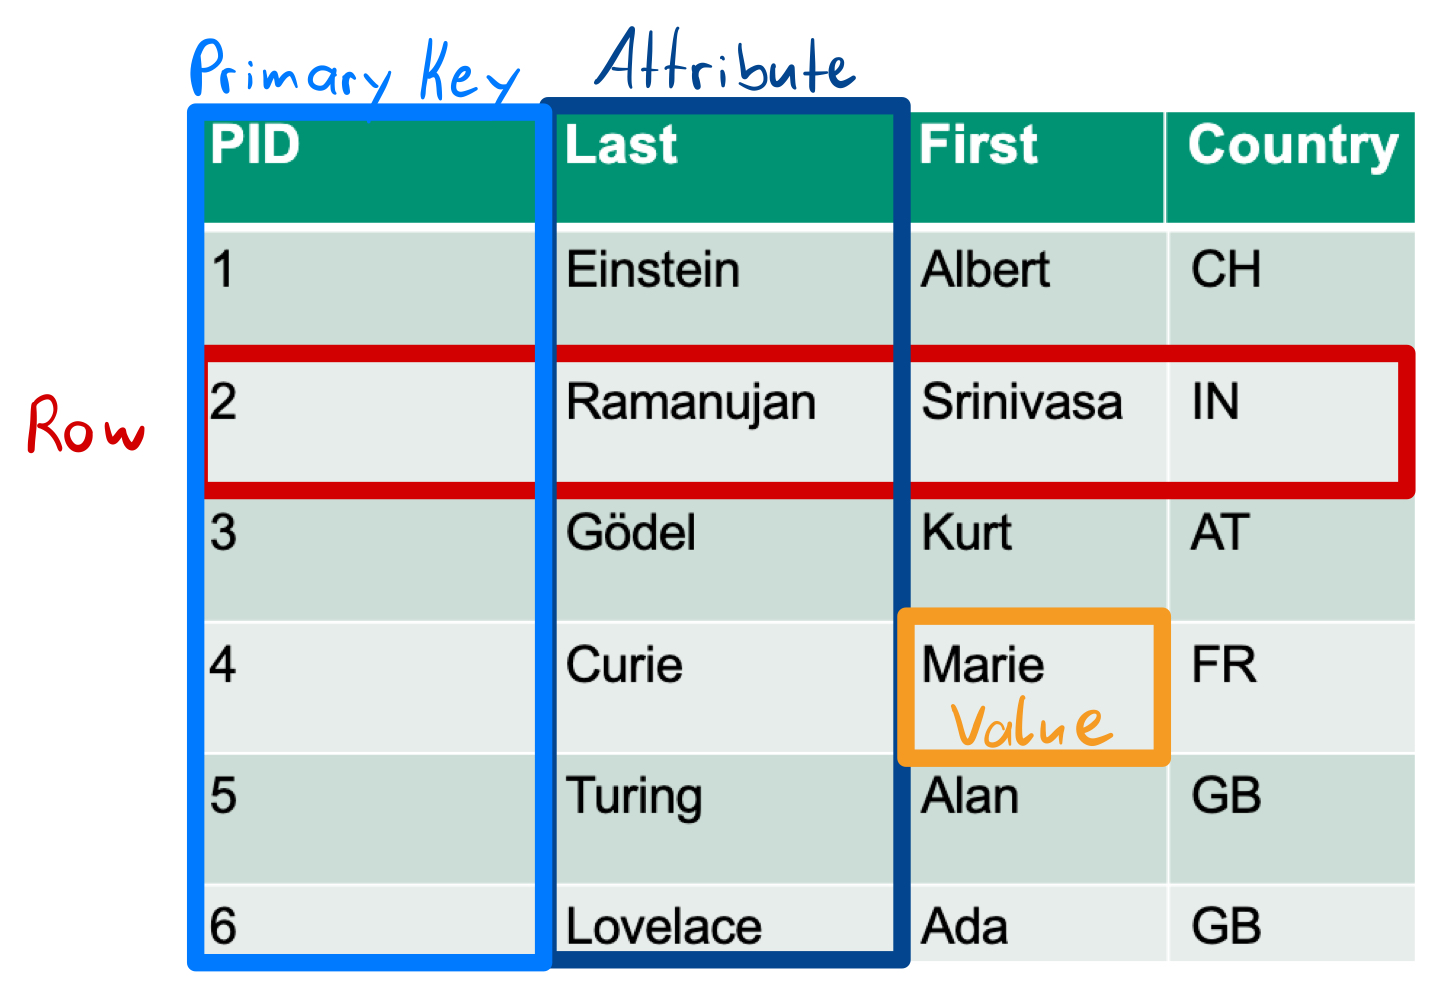
\includegraphics[width=0.7\textwidth]{Figures/Tables.jpeg}
    \caption{Table}\label{fig:table}
\end{figure}

\paragraph{Relational Integrity}
is best explained by an example such as in \cref{fig:RelInteg}.

\begin{figure}[h]
    \centering
    \begin{subfigure}{0.45\textwidth}
        \centering
        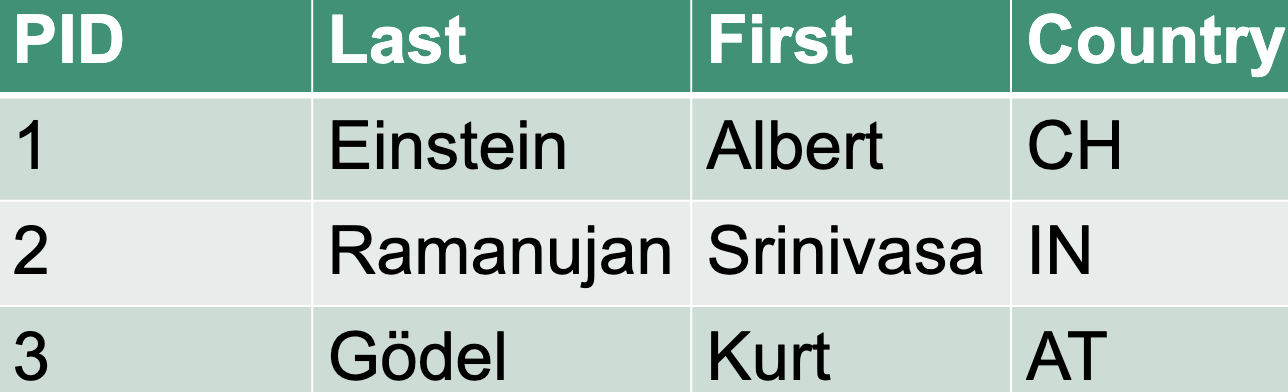
\includegraphics[width=\textwidth]{Figures/RelationalIntegrityTrue.png}
        \caption{Relational Integrity is respected.}
    \end{subfigure}
    \hfill
    \begin{subfigure}{0.5\textwidth}
        \centering
        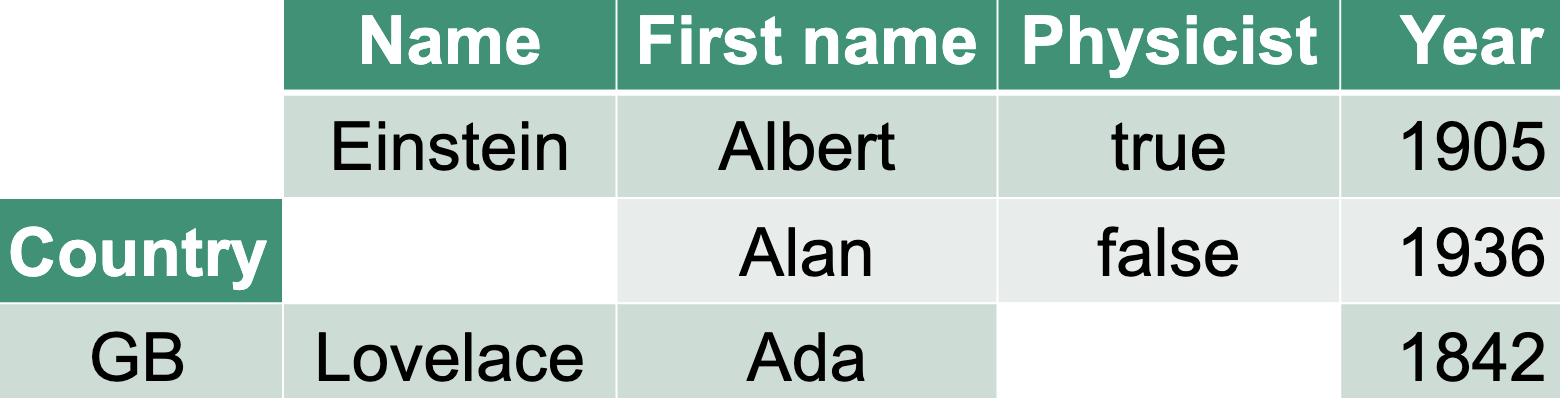
\includegraphics[width=\textwidth]{Figures/RelationalIntegrityFalse.png}
        \caption{Relational Integrity is not respected.}
    \end{subfigure}
    \caption{Examples of Relational Integrity.}\label{fig:RelInteg}
\end{figure}

\paragraph{Domain Integrity}
A table fulfills domain integrity if the values associated with each attribute are restricted to a domain. Colloquially: Each entry in an attribute column must be of the same type (character, boolean, integer,\dots).

\paragraph{Atomic Integrity}
Values in a table cannot be tables themselves. They must be atomic values.

\vspace{1\baselineskip}

The language SQL fulfills all of the three above mentioned criteria.


\subsubsection{Relational Algebra}

\paragraph{Set Queries} act on relational tables as sets. One can take the union or intersection of two sets or subtract a set from another. These operators directly and naturally translate to relational tables.

\paragraph{Filter Queries} These operators take a portion of a table: some or all columns, some or all rows, etc. They are known as projection and selection. There also exists a fancy operator called the "extended projection" that can be used to add more computed columns.

\paragraph{Renaming Queries} These operators can rename columns. Relation renaming and Attribute renaming.

\paragraph{Joining Queries} These operators can take the Cartesian product of two tables, potentially filtering to match values from both sides (join).

\paragraph{Suffling Queries} Grouping and Sorting.

\vspace{1\baselineskip}

Explanations of the previously mentioned queries:

\paragraph{Selection}
A selection takes a subset of the records belonging to the table. (A subset of the rows)

\paragraph{Projection}
A projection keeps all records, but removes columns. (A subset of the columns)

\paragraph{Grouping}
Also called aggregation, merges records by grouping on some attributes, and aggregating on all others.

\paragraph{Sorting}
Sort rows by a certain condition. E.g. alphabetic ordering of one of the attributes.

\paragraph{Cartesian Product}
A cartesian product combines each tuple from the left relational table with each tuple from the right relational table. An example can be seen in \cref{fig:CartProd}.

\begin{figure}[h!]
    \centering
    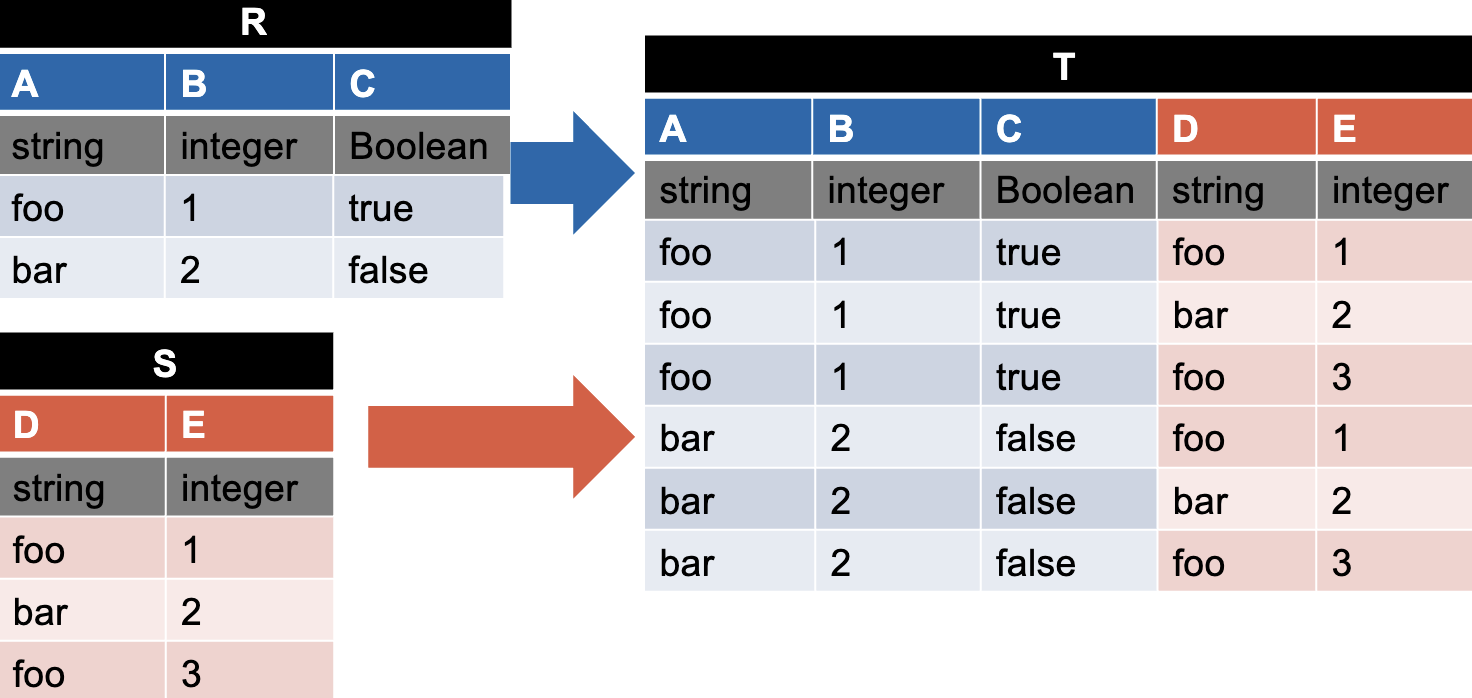
\includegraphics[width=0.7\textwidth]{Figures/CartesianProduct.png}
    \caption{Cartesian product $T = R \times S$}\label{fig:CartProd}
\end{figure}

\paragraph{Join}
A Join can be understood as a "filtered Cartesian Product" in which we only combine directly related tuples and omit all other non-matching pairs. An example can be seen in \cref{fig:Join}.
\begin{figure}[h!]
    \centering
    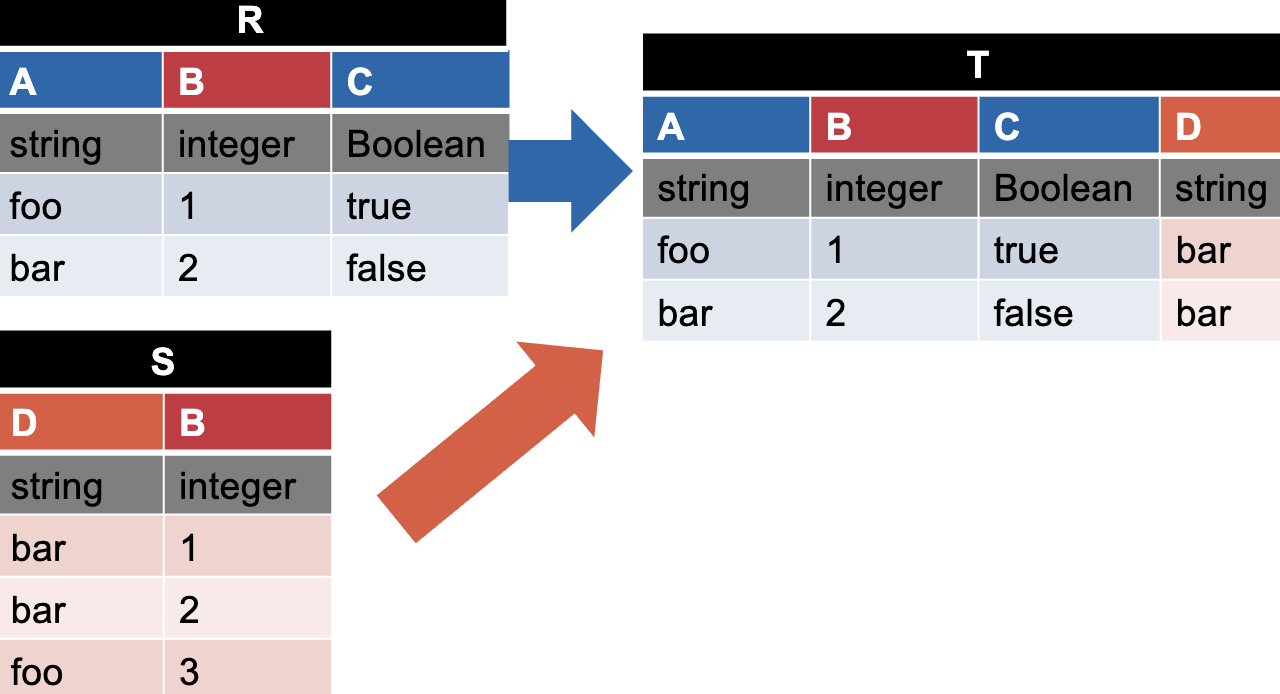
\includegraphics[width=0.7\textwidth]{Figures/Join.png}
    \caption{Join $T = R \Join S$}\label{fig:Join}
\end{figure}


\subsection{SQL}
An example that uses the most important queries can be seen in \cref{fig:SQLExmpl}.
\begin{figure}[H]
    \centering
    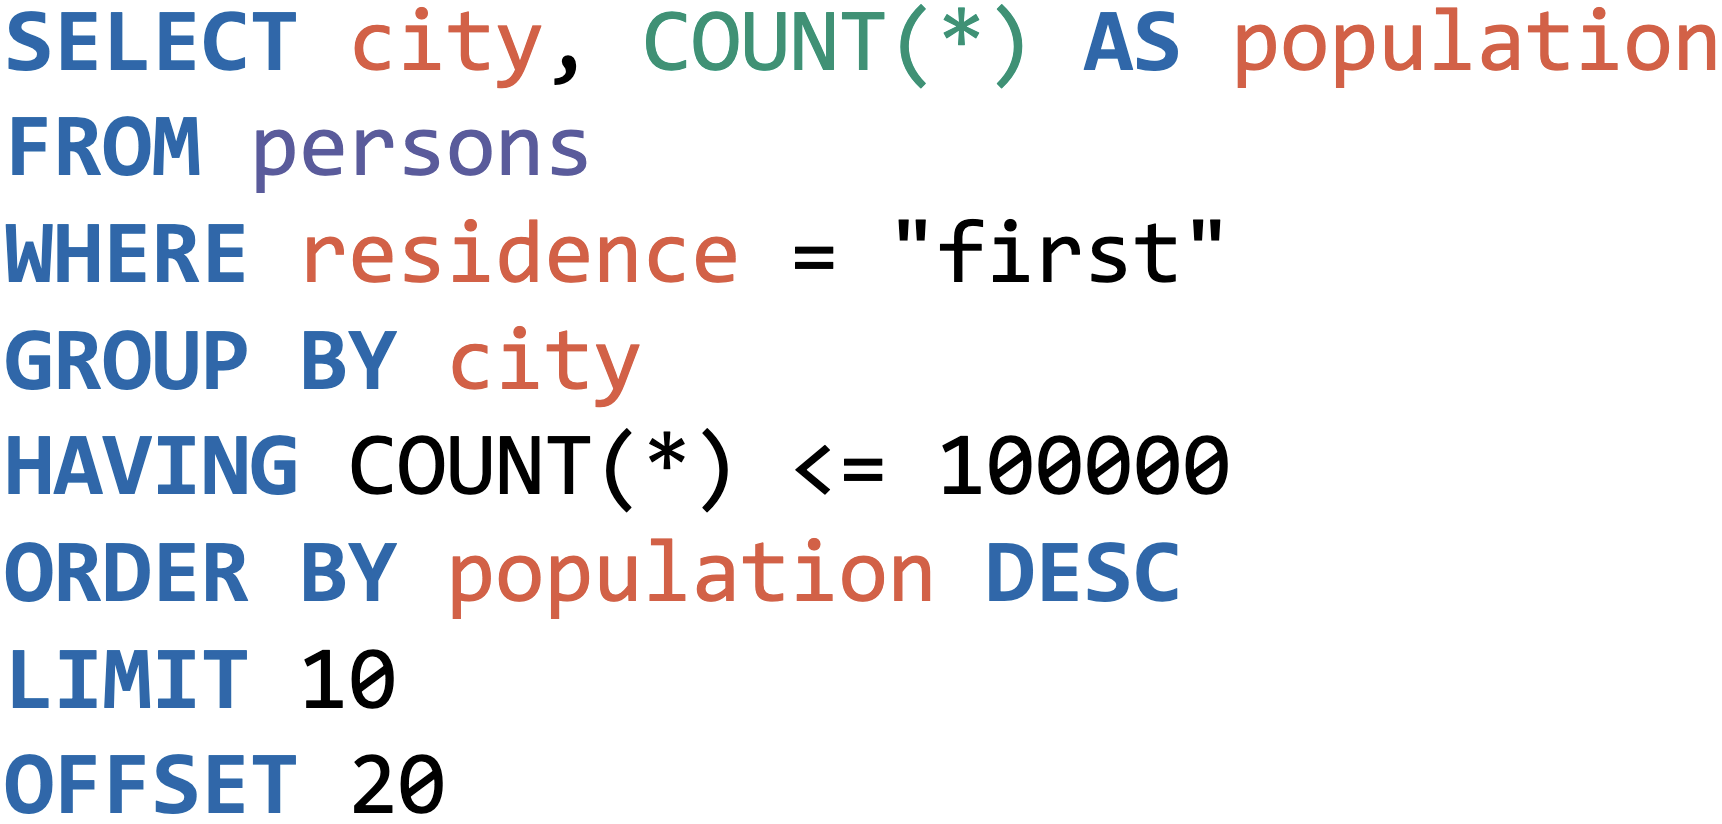
\includegraphics[width=0.5\textwidth]{Figures/ExampleSQL.png}
    \caption{Example of SQL code.}\label{fig:SQLExmpl}
\end{figure}
The SELECT clause selects which attributes of the table we want to use. We can use AS to rename certain attributes. The FROM clause selects from which tables to read the data. The WHERE clause performs a selection. The GROUP BY clause performs an aggregation. The HAVING clause is like the WHERE clause, but performs the selection after, rather than before, the grouping. The ORDER BY clause reorders the output rows according to the specified key. DESC specifies that it should be ordered in descending order. The LIMIT and OFFSET clauses allow pagination of the output: OFFSET specifies how many records (rows) to skip, and LIMIT specifies how many records (rows) to output after the skipped ones.
All clauses are optional except for SELECT and FROM.

More examples can be seen in \cref{lst:SQLExamples1}. Union queries merge two tables and duplicates are eliminated. Theta Joins are realted to normal forms. High normal form means, that we have more smaller tables. Conversely, if we have low normal forms, we have one large table with all the data. In a Theta Join, if there is match in the specified condition in the two tables, the rows are merged (one row gets more attributes). In a Full outer Join, two tables get merged just like in the Theta Join, just that all rows are added to the new table, and if there is no match in the specified condition to join, the new attributes of that row will be filled with NULL values. Natural Joins join two tables in the most natural way. No specific condition needs to be specified here.

If it is not cleare what these queries do, refer to the slides \textit{02 - Big Data - Lessons Learnt}.

\begin{lstlisting}[style=sql, caption={SQL code examples}, label={lst:SQLExamples1}]
    -- A Union Query
    SELECT * FROM TableName1 UNION SELECT * FROM TableName2;

    -- Theta Joins
    SELECT *
    FROM TableName1 JOIN TableName2
        ON TableName1.Attribute1 = TableName2.Attribute2

    -- Full outer Joins
    SELECT *
    FROM TableName1 FULL OUTER JOIN TableName2
        ON TableName1.Attribute1 = TableName2.Attribute2

    -- Natural Join
    SELECT *
    FROM TableName1 NATURAL JOIN TableName2

    -- Nesting
    SELECT attribute1, attribute2
    FROM (
        SELECT TableName1.attribute1 AS attr1,
               attribute2,
               attribute3,
               TableName2.attribute1 as attr2
               attribute 4
        FROM TableName1 FULL OUTER JOIN TableName2 USING attribute 2
    )
\end{lstlisting}

There are three-valued logics in SQL. These three values are TRUE, FALSE and UNKNOWN.

\subsection{Languages}
There are Data Manipulation Languages (DML) (e.g. query, insert, remove rows) and Data Definition Languages (DDL) (e.g. Create or table/scheme, drop it).

There are six main categories of languages: assembly code, functional and declarative languages (SQL, JSONiq, SPARQL), co-habiting with lower level APIs an. Another one are machine learning frameworks.

\paragraph{Good to know}
OnLine Transaction Processing (OLTP) is write-intensive and used if you have to modify the data a lot. Here, it is useful to use higher normal forms because you do not want to use large tables.

OnLine Analytical Processing (OLAP) is read-intensive and used for applications of Big data. Here you want to work with large dataframes. That means, we work with low normal forms.


\subsection{Transactions}
There are four main properties (ACID) that the good old systems provide:

\paragraph{Atomicity}Either an update (called a transaction if it consists of several updates) is applied to the database completely, or not at all.

\paragraph{Consistency} Before and after the transactions, the data is in a consistent state.

\paragraph{Isolation} The system "feels like" the user is the only one using (writing to) the system (databasis), where in fact maybe thousands of people are using it as well concurrently.

\paragraph{Durability} Any data written to the database is durably stored and will not be lost.


\subsection{Scaling up and out}
What happens when we have lot of rows or columns or nestings.

